%!TEX root=./poly.tex
%
\section{\tops{$\RO(\Z_p)^\land$}{RO(Z\_p)\^}-graded \tops{$\TR$}{TR} of smooth algebras}
\label{sec:dRW}

\newcommand{\untwist}{\smash{{}^{\fade{\scriptscriptstyle\phi^{-1}}}}}
\newcommand{\thh}{\THH(S;\Z_p)}

In this section we study the polyrepresentation-graded $\TR$ of a $p$-completely smooth algebra $S$ over a perfectoid base ring $R$, deducing Norm maps for the de Rham-Witt complex as our main application. We recall the explicit description of the de Rham-Witt complex in this setting in \sec\ref{sub:dRW-perfd}. In \sec\ref{sub:ctgs}, we extend the homotopy orbits to TR spectral sequence to compute $\TR^\bullet_\rog(S;\Z_p)$ in the contiguous range. We then record some special cases in \sec\ref{sub:special}. We identify the Norm on the de Rham-Witt complex (borrowed from the Norm on $\TR$) in \sec\ref{sub:dRW-norm}.

Let us explain the strategy. As a $\T$-spectrum, the representation sphere $S^{\lambda^k}$ has a 1-step cell structure with associated graded
\[ S^0,\quad\T/C_{k+}\tnsr S^1. \]
As a $C_n$-spectrum, it instead has a 2-step cell structure with associated graded
\[ S^0,\quad C_n/C_{k+}\tnsr S^1,\quad C_n/C_{k+}\tnsr S^2. \]

The ``short'' cell structure was very effective at computing $\TCmin_\rog$ and $\TP_\rog$ in \sec\ref{sec:qrsp} since they are even. If one uses the ``long'' cell structure to compute $\TR^\bullet_\rog$, one finds that the 1-skeleton contributes $V^k$ and the 2-skeleton contributes $dV^k$ to $\Fil^k\dRW[\bullet]^*=V^k + dV^k$. While instructive, this computation is extremely messy, so we defer it to a companion paper. Instead, we will use the BMS filtration to import the results of \sec\ref{sec:qrsp} and compute $\TR^\bullet_\rog$ via the homotopy orbits to $\TR$ spectral sequence from \cite[\sec3]{ROS1TR} and \cite[\sec3]{SulROGTHH}.

\subsection{Structure of the de Rham-Witt complex over a perfectoid base}
\label{sub:dRW-perfd}

Let $R$ be a perfectoid ring, and let $S$ be a $p$-completely smooth $R$-algebra. We are interested in the relative de Rham-Witt complex $\dRW[\bullet]^*_{S/R}$ of Langer-Zink \cite{LangerZinkDRW}. We recall from \cite{BMS1} the structure of this complex and its connection to the $q$-de Rham complex.

\begin{example}[Cartier isomorphism]
  \label{ex:cartier}
  Let $R$ be a perfectoid ring admitting all $p$-power roots of unity. Fix a compatible choice of roots $\{\zeta_{p^n}\}$, and define the following elements of $A=\Ainf(R)=\rmW(R^\flat)$:
  \begin{align*}
    q &= [\epsilon] & \~\xi_n &= (p^n)_q & \xi_n &= (p^n)_{q^{1/p^{n+1}}}\\
    \mu &= 1-q &&= \frac{\phi^n(\mu)}\mu &&= \frac{\phi^{-1}(\mu)}{\phi^{-(n-1)}(\mu)}
  \end{align*}
  In this context, prismatic cohomology of $R$-algebras can be computed as a $q$-de Rham complex by \cite[Lemma 9.6]{BMS1} and \cite[Theorem 17.2]{Prismatic}.

  We work this out for the affine line $S=R[x]^\land_p$. The $q$-de Rham complex is given by
  \[ \AOmega_S = \widehat{\bigoplus_n} \left[A{\<x^n\>} \xra{\nabla_q} A{\<x^n\dlog x\>}\right] \]
  where $\widehat\bigoplus$ denotes a $p$-completed direct sum, and the differential sends $\nabla_q(x^n) = (n)_q x^n \dlog x$.

  Let us compute the cohomology of $\~\Omega_S = \AOmega_S/\~\xi = \AOmega_S/(p)_q$. Now the differential is $0$ for exponents divisible by $p$, and an isomorphism otherwise. We conclude that
  \begin{align*}
    \H^*(\~\Omega_S) &= \widehat{\bigoplus_n} A/\~\xi{\<x^{pn}\>}[0] \oplus A/\xi{\<x^{pn}\dlog x\>}[-1]
  \end{align*}
  These are isomorphic to
  \[\xymatrix@R=2em@C=-4em{
      *!R{A/\xi{\<x^n\>}\ } \ar[r]^-\phi_-\sim & *!L{A/\~\xi{\<x^{pn}\>}}\\
      *!R{A/\xi{\<x^n\dlog x\>}\tnsr \xi^{-1}\ } \ar[r]^-\phi_-\sim & *!L{A/\~\xi{\<x^{pn}\dlog x\>}}
  }\]
  The twist by $\xi^{-1}$ is necessary in the second line because $\phi(\dlog x)=\~\xi\dlog x$. In other words,
  \[ \H^*(\~\Omega_S) = \Omega^*_{S/R}\{-*\}=\Omega^*_{S/R}\tnsr \xi^{-*}A, \]
  in accordance with \cite[Theorem 8.7]{BMS1}.

Next we compute the cohomology of $\widetilde{\dRW[1]}_S = \AOmega_S/\~\xi_2 = \AOmega_S/(p^2)_q$. We find that
  \begin{align*}
    \H^*(\widetilde{\dRW[1]})
      &= \phantom{{}\oplus} \bigoplusp_n A/\~\xi_2\<x^{p^2 n}\>[0] \oplus A/\~\xi_2\<x^{p^2 n}\dlog x\>[-1]\\
      &\phantom{{}=} \oplus \bigoplusp_{p\nmid j} A/\~\xi\<\phi(\~\xi) x^{pj}\>[0] \oplus A/\~\xi\<x^{pj}\dlog x\>[-1].
  \end{align*}
  These are isomorphic to
  \[\xymatrix@R=2em@C=-5em{
      *!R{A/\xi_2\<x^n\>\ } \ar[r]^-{\phi^2}_-\sim & *!L{A/\~\xi_2\<x^{p^2n}\>}\\
      *!R{A/\phi^{-1}(\xi)\<\xi x^{j/p}\>\ } \ar[r]^-{\phi^2}_-\sim & *!L{A/\~\xi\<\phi(\~\xi) x^{pj}\>}\\
      *!R{A/\xi_2\<x^n\dlog x\>\tnsr \xi_2^{-1}\ } \ar[r]^-{\phi^2}_-\sim & *!L{A/\~\xi_2\<x^{p^2n}\dlog x\>}\\
      *!R{A/\phi^{-1}(\xi)\<x^{j/p}\dlog x\>\tnsr \xi_2^{-1}\ } \ar[r]^-{\phi^2}_-\sim & *!L{A/\~\xi\<x^{pj}\dlog x\>}
  }\]
  In other words, $\H^*(\widetilde{\dRW[1]}_S) = \dRW[1]^*_{S/R}\{-*\}=\dRW[1]^*_{S/R} \tnsr \xi_2^{-*}A$, in accordance with \cite[Theorem 11.1]{BMS1}.
\end{example}

We need a similar calculation which is not covered by \cite[Theorem 11.1]{BMS1}.

\begin{proposition}
  \label{prop:h*-nyg}
  If $S$ is a $p$-completely smooth $R$-algebra, then
  \[
    \H^j\left(\frac{\Nyg^{\ge i}\AOmega_S}{I_n \Nyg^{\ge i+1}\AOmega_S}\right)
    =
    \left\{
      \begin{array}{r@{}ll}
        \dRW[n]^j_{S/R} &{}\tnsr \xi_{n+1}^{-j} \phi^{-n}(\xi)^{i}A & i\ge j\\
        \dRW[n-1]^j_{S/R} &{}\tnsr \xi_n^{-j}A & i < j
      \end{array}
    \right.
  \]
\end{proposition}
\begin{proof}
  By \cite[Remark 9.11]{BMS2}, the Nygaard filtration is given explicitly by
  \[ \Nyg^{\ge i}\AOmega^j_S = \xi^{\pos{i-j}}\AOmega^j_S \]
  where $\pos x \defeq \max(x, 0)$. If $i<j$, then this is just $\H^j(\AOmega_S/I_n)=\dRW[n-1]^j_{S/R} \tnsr \xi_n^{-j}A$ by the existing Cartier isomorphism \cite[Theorem 11.1]{BMS1}. For $j \le i$, the Frobenius induces an equivalence
  \[ \tau^{\le j} \Nyg^{\ge i} \AOmega_S \morph^\varphi_\sim \tau^{\le j} I^i A\Omega_S \]
  by (applying $\tau^{\le j}$ to both sides of) \cite[Theorem 2.16]{BouisCartier}. Thus we get
  \begin{align*}
    \H^j\left(\frac{\Nyg^{\ge i}\AOmega_S}{I_n\Nyg^{\ge i+1}\AOmega_S}\right)
    &= \H^j\left(\frac{\tau^{\le j}\Nyg^{\ge i}\AOmega_S}{\tau^{\le j+1}I_n\Nyg^{\ge i+1}\AOmega_S}\right)\\
    &\morph^\varphi_\sim \H^j\left(\frac{\tau^{\le j}I^i\AOmega_S}{\tau^{\le j+1}I^i I_{n+1}\AOmega_S}\right)\\
    &= \H^j\left(\frac{\AOmega_S}{I_{n+1}\AOmega_S}\right) \tnsr I^i\\
    &\xra[\sim]{\phi^{-{n+1}}} \dRW[n]^j_{S/R} \tnsr \xi_{n+1}^{-j}A \tnsr \phi^{-n}(\xi)^i A. \qedhere
  \end{align*}
\end{proof}

\begin{proofsketch}
  We sketch a modern proof of Hesselholt's theorem, as formulated in Notation \ref{not:canonical}:
  \[ \TR^n_{2i,j}(S;\Z_p) = \dRW[n]^j_{S/R} \tnsr \xi_{n+1}^i A. \]

  The base case $n=0$ is \cite[Corollary 6.9]{BMS2}. Inductively, we consider the isotropy separation square
  \[\xymatrix{
      \TR^n(S;\Z_p) \ar[r]^-R \ar[d] \pullback & \TR^{n-1}(S;\Z_p) \ar[d]\\
      \thh^{hC_{p^n}} \ar[r] & \thh^{tC_{p^n}}
  }\]
  By \cite[Lemma 3.1]{RiggenbachTruncated}, the motivic filtrations are
  \begin{align*}
    \gr^i_\mot \thh^{hC_{p^n}}
      &= \frac{\Nyg^{\ge i}\hat\prism_S}{\~\xi_n \tnsr \Nyg^{\ge i+1}\hat\prism_S}\tnsr \~\xi_n^i A[2i]\\
      &= \frac{\Nyg^{\ge i}A\Omega_S}{\~\xi_n \tnsr \Nyg^{\ge i+1}A\Omega_S}\tnsr \~\xi_n^i A[2i]\\
    \gr^i_\mot \thh^{tC_{p^n}}
      &= \frac{\hat\prism_S}{\~\xi_n}\tnsr \~\xi_n^i A[2i]\\
      &= \frac{A\Omega_S}{\~\xi_n}\tnsr \~\xi_n^i A[2i]\\
      &= \~{\dRW[n-1]_S}\tnsr \~\xi_n^i A[2i]\\
  \end{align*}
  Taking cohomology and applying the Cartier isomorphism (\cite[Theorem 8.7]{BMS1} and Proposition \ref{prop:h*-nyg}), we find that $\thh^{hC_{p^n}}_*$ is computed by the following $E_1$ spectral sequence:
  \[\xymatrix@C=1em@R=1em{
      \fade\dots & \fade{\dRW[n-1]^5 \tnsr \xi_n^{-3}} & \fade{\dRW[n-1]^4 \tnsr \xi_n^{-2}} & \fade{\dRW[n-1]^3 \tnsr \xi_n^{-1}} & \dRW[n]^2 & \dRW[n]^1 \tnsr \xi_{n+1} \\
      \fade\dots & \fade{\dRW[n-1]^3 \tnsr \xi_n^{-2}} & \fade{\dRW[n-1]^2 \tnsr \xi_n^{-1}} & \dRW[n]^1 & \dRW[n]^0 \tnsr \xi_{n+1}\\
      \fade{\dRW[n-1]^2 \tnsr \xi_n^{-2}} &\fade{\dRW[n-1]^1 \tnsr \xi_n^{-1}} &
      \dRW[n]^0 \ar@[lightgray][ul]\\
    \fade{\dRW[n-1]^0 \tnsr \xi_n^{-1}}\\
      \dots & \pi_{-1} & \pi_0 & \pi_1 & \pi_2 & \dots
  }\]
  Observe how the negative twists from the Cartier isomorphism cancel out the Breuil-Kisin twists from the motivic filtration, shifting de Rham-Witt terms from cohomological to homological degree. Hesselholt's proof \cite{LarsPTyp} based on the cyclic bar construction establishes an additive decomposition which shows that there are no further differentials or extensions (although it should be possible to give a direct proof within the current formalism).

  The solid region is where $\TR^{n-1}_* \to \THH^{tC_{p^n}}_*$ is an isomorphism, which implies the same for $\TR^n_* \to \THH^{hC_{p^n}}_*$; and the faded region is an isomorphism for $\THH^{hC_{p^n}} \to \THH^{tC_{p^n}}$, which implies the same for $\TR^n_* \to \TR^{n-1}_*$. Hesselholt's theorem follows. \qed
\end{proofsketch}

\subsection{Contiguous range}
\label{sub:ctgs}

In this section we compute $\TR_\rog(S; \Z_p)$ in the contiguous range. Our method is the homotopy orbits to TR spectral sequence from \cite{ROS1TR,SulROGTHH}. In fact, the computation for $\TR_{\rog,j}(S;\Z_p)$ works the same way as the computation for $\TR_\rog(R;\Z_p)$.

\begin{method}
  We explain the strategy for computing $\TR^1_\rog(S;\Z_p)$. We will use the isotropy separation square
  \begin{equation}
    \label{eq:isotropy}
    \vcenter{\xymatrix{
      \TR^1(S;\Z_p) \ar[r] \ar[d] \pullback & \thh^{\Phi C_p} \ar[d]\\
      \thh^{hC_p} \ar[r] & \thh^{tC_p}
    }}
  \end{equation}
  Recall that with this method, the computation breaks up as a direct sum over de Rham-Witt degrees $j$, where $\pi_{\alpha,j}$ denotes the $\dRW^j$ contribution to $\pi_{\alpha+j}$. With this notation, the spectral sequence associated to the isotropy separation square takes the form
  \begin{align*}
    E_0 &=\dbox{$\vcenter{\xymatrix@R=0.2em{
          \thh^{tC_p}_{\alpha,j} & \thh^{hC_p}_{\alpha,j} \ar[l]\\
                              & \thh^{\Phi C_p}_{\alpha,j}
                   }}$}\\
    E_1 &=
    \dbox{$\vcenter{\xymatrix@R=0.2em{
    (\thh_{hC_p})_{\alpha-1,j} & (\thh_{hC_p})_{\alpha,j} \\
                            & \thh^{\Phi C_p}_{\alpha,j} \ar[ul]^-\varphi
                                                               }}$}\\
    E_\infty &=
    \dbox{$\vcenter{\xymatrix@R=0.2em{
    \TR^1_{\alpha-1,j}(S;\Z_p) & \gr^1 \TR^1_{\alpha,j}(S;\Z_p)\\
                               & \gr^0\TR^1_{\alpha,j}(S;\Z_p)
                                    }}$}
  \end{align*}

  We need to identify these terms canonically. Suppose that $\alpha=(d_0;d_\infty)$ is a complex $C_p$-representation. Since the Euler class $a_\lambda$ is invertible in the right column of \eqref{eq:isotropy}, the corresponding groups canonically depend only on $d_\infty$: we have canonical identifications
  \begin{align*}
    \thh^{\Phi C_p}_{\alpha,j} &= \thh^{\Phi C_p}_{2d_\infty,j}\\
                               &= \begin{cases}
                                 \Omega^j_{S/R} \tnsr \xi^{d_\infty} & d_\infty \ge 0\\
                                 0 & d_\infty < 0,
                               \end{cases}\\
    \thh^{tC_p}_{\alpha,j} &= \thh^{t C_p}_{2d_\infty,j} \\
                           &= \widetilde{\Omega}^j_{S/R} \tnsr \xi^{d_\infty}.
  \end{align*}
  
  Since the Thom class $u_\lambda$ is invertible in the bottom row of \eqref{eq:isotropy} (and in particular on $\thh_{hC_p}$), the corresponding groups \emph{non-canonically} depend only on $d_0$: we have \emph{non-canonical} identifications
  \begin{align*}
    \thh^{hC_p}_{\alpha,j} &\mathrel{\red\isom} \thh^{hC_p}_{2d_0,j}\\
                           &= \left\{\!\!\!
                             \begin{array}{r@{}ll}
                               \dRW[1]^j_{S/R} &{}\tnsr (\xi\phi^{-1}(\xi))^{d_0} & d_0\ge0\\
                               \Omega^j_{S/R} &{}\tnsr \xi^{d_0} & d_0<0
                           \end{array}\right.
  \end{align*}
  To make this canonical, we need to match the twist on $\thh^{tC_p}$. The map
  \[ \thh^{hC_p}_{2d_0,j} \morph \thh^{tC_p}_{2d_0,j} \]
  is $\phi^{-1}(\xi)^{d_0}$ times the canonical projection when $d_0\ge 0$, and an isomorphism when $d_0<0$. Thus, the canonical identification is
  \[
    \THH^{hC_p}_{\alpha,j} =
    \left\{\!\!\!
      \begin{array}{r@{}ll}
        \dRW[1]^j_{S/R} &{}\tnsr \xi^{d_0} \phi^{-1}(\xi)^{d_\infty} & d_0\ge 0\\
        \Omega^j_{S/R} &{}\tnsr \xi^{d_\infty} & d_0 < 0
    \end{array}
    \right.
  \]

  Finally, we switch to poly-representation notation: if $\alpha = (d_0;d_\infty)$ is a $\T$-representation, the corresponding $\Z_p$-polyrepresentation is $\m\alpha=(\m d_0, \m d_1)$ with $\m d_0=d_\infty$ and $\m d_1 = d_0$. Thus our canonical identifications are
  \[
    \dbox{$\vcenter{\xymatrix@R=0.2em{
          \thh^{tC_p}_{\alpha,j} & \thh^{hC_p}_{\alpha,j} \\
                              & \thh^{\Phi C_p}_{\alpha,j}
                   }}$}
    =
    \dbox{$\vcenter{\xymatrix@R=0.2em@C=-4em{
          \Omega^j_{S/R} \tnsr \xi^{\m d_0} & *!L{\begin{cases}\dRW[1]^j_{S/R} \tnsr \xi^{\m d_0} \phi^{-1}(\xi)^{\m d_1} & \m d_1 \ge 0\\ 
              \Omega^j_{S/R} \tnsr \xi^{\m d_0} & \m d_1 < 0
                                      \end{cases}} \\
                                      & *!L{\begin{cases}\Omega^j_{S/R} \tnsr \xi^{\m d_0} & \m d_0 \ge 0\\ 
                                          0 & \m d_0 < 0
                                      \end{cases}}
                                                               }}$}
      \]
\end{method}

\begin{example}
  First we compute $\TR^1_\rog(S\rel\SAinf{R^+})$ when $R^+$ is a $p$-torsionfree perfectoid ring and $S$ is a $p$-completely smooth $R^+$-algebra. Let $\m\alpha = (\m d_0,\m d_1)$ be a virtual $\Z/p$-polyrepresentation. There are three cases, depending on the signs of $\m d_0$ and $\m d_1$ (the result is zero if both are negative).

  \begin{center}
    \begin{tabular}{c|c}
      (1) & (2)\\\hline
      0 & (3)
    \end{tabular}
  \end{center}

  \begin{enumerate}
    \item $\m d_0\ge0$, $\m d_1<0$:
      \[
        \left(\vcenter{\xymatrix@R=0em{
              \Omega^j \tnsr \xi^{\m d_0} & \Omega^j \tnsr \xi^{\m d_0} \ar[l]_-\sim\\
                                          & \Omega^j \tnsr \xi^{\m d_0}
        }}\right)
        \leadsto
        \left(\vcenter{\xymatrix@R=0em{
              \phantom0 & \phantom0\\
               & \Omega^j \tnsr \xi^{\m d_0}
        }}\right)
      \]
      In this region, $\TR^1_\rog$ coincides with $\THH^{\Phi C_p}_\rog$.

    \item $\m d_0\ge 0$, $\m d_1\ge 0$: since $\rmW_0(R^+)=A/\xi$ is $\phi^{-1}(\xi)$-torsionfree,
      \begin{align*}
        &\phantom{{}\leadsto}\left(\vcenter{\xymatrix@R=0em{
        \Omega \tnsr \xi^{\m d_0} & {\dRW[1]^j \tnsr \xi^{\m d_0} \phi^{-1}(\xi)^{\m d_1}} \ar[l]\\
                                        & {\Omega^j \tnsr \xi^{\m d_0}}
        }}\right)\\
        &\leadsto
        \left(\vcenter{\xymatrix@R=0em{
          \dfrac{\Omega^j}{\phi^{-1}(\xi)^{\m d_1}} \tnsr \xi^{\m d_0} & \Fil^1\dRW[1]^j \tnsr \xi^{\m d_0} \phi^{-1}(\xi)^{\m d_1}\\
                                                                  & \Omega^j \tnsr \xi^{\m d_0} \ar[ul]
        }}\right)\\
        &\leadsto
        \left(\vcenter{\xymatrix@R=0em@C=10em{
        \phantom0 & *!R{\Fil^1\dRW[1]^j \tnsr \xi^{\m d_0} \phi^{-1}(\xi)^{\m d_1}}\\
              \phantom0 & *!R{\Omega^j \tnsr \xi^{\m d_0} \phi^{-1}(\xi)^{\m d_1}}
        }}\right)
      \end{align*}
      The extension is $\dRW[1]^j_{S/R^+} \tnsr \xi^{\m d_0} \phi^{-1}(\xi)^{\m d_1}$. In this region, $\TR^1_\rog$ coincides with $\THH^{hC_p}_\rog$.

    \item $\m d_0<0$, $\m d_1\ge0$: again using that $R^+$ is $\phi^{-1}(\xi)$-torsionfree,
      \[
        \left(\vcenter{\xymatrix@R=0em{
          \Omega \tnsr \xi^{\m d_0} & {\dRW[1]^j \tnsr \xi^{\m d_0} \phi^{-1}(\xi)^{\m d_1}} \ar[l]\\
        }}\right)
        \leadsto
        \left(\vcenter{\xymatrix@R=0em{
              \dfrac{\Omega^j}{\phi^{-1}(\xi)^{\m d_1}} \tnsr \xi^{\m d_0} & \Fil^1\dRW[1]^j \tnsr \xi^{\m d_0} \phi^{-1}(\xi)^{\m d_1}
        }}\right)
      \]
      In this region, $\TR^1_\rog$ coincides with $(\THH_{hC_p})_\rog$.
  \end{enumerate}

  In summary:
  \begin{center}
    \renewcommand{\arraystretch}{2} 
    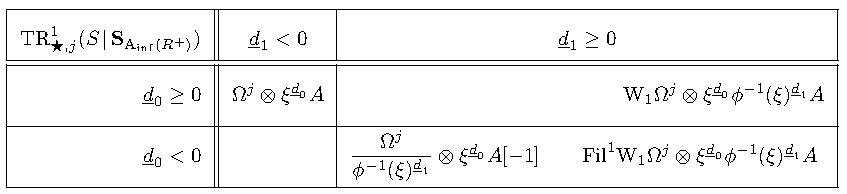
\includegraphics[width=0.85\textwidth]{tables/summary-perfd.pdf}
    % \begin{tabular}{|r||c|r|}
    % \firsthline
    % $\TR^1_{\rog,j}(S\rel\SAinf{R^+})$ & $\m d_1 <0$ & \multicolumn{1}{c|}{$\m d_1\ge 0$}\\\hline\hline
    %                               \pad $\m d_0\ge 0$ & $\Omega^j \tnsr \xi^{\m d_0}A$ & $\dRW[1]^j \tnsr \xi^{\m d_0}\phi^{-1}(\xi)^{\m d_1}A$\\[.5em]\hline
    %                               \pad $\m d_0<0$ && $\dfrac{\Omega^j}{\phi^{-1}(\xi)^{\m d_1}}\tnsr\xi^{\m d_0}A[-1] \qquad \Fil^1\dRW[1]^j \tnsr \xi^{\m d_0}\phi^{-1}(\xi)^{\m d_1}A$
    %                               \\[.5em]\hline
    % \end{tabular}
  \end{center}
\end{example}

For an arbitrary perfectoid ring $R$, the argument in the first region goes through. In the second region, the intermediate pages may look different, but the final answer is the same: regardless of $R$, $\THH^{\Phi C_p}_\rog \to \THH^{tC_p}_\rog$ is an isomorphism in this region, so a priori so must be $\TR^1_\rog \to \THH^{hC_p}_\rog$. The third region (as well as the $E^1$ page of the second region) depends more delicately on the $p$-torsion of $R$.

\begin{example}
  Next we compute $\TR^1_{\rog,j}(S\rel\SW k)$ when $k$ is a perfect $\F_p$-algebra and $S$ is a smooth $k$-algebra. By the preceding remark, it suffices to consider the second region. Note that
  \begin{align*}
    \ker\left(\dRW[1]^j \tnsr p^{\m d_0 + \m d_1} \to \Omega^j \tnsr p^{\m d_0} \right)
    &=
    \begin{cases}
      \Fil^1 \dRW[1]^j \tnsr p^{\m d_0 + \m d_1} & \m d_1 = 0\\
      \phantom{\Fil^1} \dRW[1]^j \tnsr p^{\m d_0 + \m d_1} & \m d_1 > 0
    \end{cases}\\
    &= \Fil^{1 - \m d_1} \dRW[1]^j \tnsr p^{\m d_0 + \m d_1}
  \end{align*}
  recalling that by convention $\Fil^r \dRW[\bullet]^* = \dRW[\bullet]^*$ for $r\le0$. This may look strange, but it will prevent us from losing our minds with casework. We similarly have the peculiar identity
  \[ \ker\left( \Omega^j \to \frac{\Omega^j}{p^{\m d_1}} \right) = \dRW[-\m d_1]^j \tnsr p^{\m d_1}W \]
  where the right-hand side is zero for $\m d_1>0$.

  Now the spectral sequence goes
  \begin{align*}
    &\phantom{{}\leadsto}\left(\vcenter{\xymatrix@R=0em{
    \Omega \tnsr p^{\m d_0} & {\dRW[1]^j \tnsr p^{\m d_0 + \m d_1}} \ar[l]\\
                                    & {\Omega^j \tnsr p^{\m d_0}}
    }}\right)\\
    &\leadsto
    \left(\vcenter{\xymatrix@R=0em{
  \dfrac{\Omega^j}{p^{\m d_1}} \tnsr p^{\m d_0} & \Fil^{1-\m d_1}\dRW[1]^j \tnsr p^{\m d_0 + \m d_1}\\
                                                              & \Omega^j \tnsr p^{\m d_0} \ar[ul]
    }}\right)\\
    &\leadsto
    \left(\vcenter{\xymatrix@R=0em@C=10em{
 \phantom0 & *!R{\Fil^{1 - \m d_1}\dRW[1]^j \tnsr p^{\m d_0 + \m d_1}}\\
 \phantom0 & *!R{\dRW[-\m d_1]^j \tnsr p^{\m d_0} }
    }}\right)
  \end{align*}
  and the extension is $\dRW[1]^j_S \tnsr p^{\m d_0 + \m d_1}W$.

  In summary:
  \begin{center}
    \renewcommand{\arraystretch}{2} 
    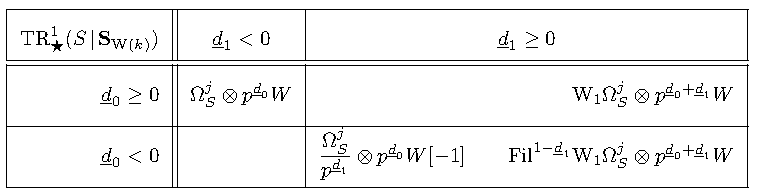
\includegraphics[width=0.76\textwidth]{tables/summary-crys.pdf}
  % \begin{tabular}{|r||c|r|}
  % \firsthline
  % $\TR^1_\rog(S\rel\SW k)$ & $\m d_1 <0$ & \multicolumn{1}{c|}{$\m d_1\ge 0$}\\\hline\hline
  %   \pad $\m d_0\ge 0$ & $\Omega^j_S \tnsr p^{\m d_0}W$ & $\dRW[1]^j_S \tnsr p^{\m d_0+\m d_1}W$\\[.5em]\hline
  %   \pad $\m d_0<0$ && $\dfrac{\Omega^j_S}{p^{\m d_1}}\tnsr p^{\m d_0}W[-1] \qquad \Fil^{1-\m d_1}\dRW[1]^j_S \tnsr p^{\m d_0 + \m d_1}W$\\[.5em]\hline
  %  \end{tabular}
\end{center}
\end{example}

\begin{example}
  We can also compute these as Mackey functors. The basic Mackey functors in play are
  \[\xymatrix{
      0 \ar[r] & \Fil^1\dRW[1]^j \mdown F \ar[r] & \dRW[1]^j \mdown F \ar[r] & \Omega^j \mdown{} \ar[r] & 0 \\
      0 \ar[r] & \Omega^j \ar@{=}[r] \mup V & \Omega^j \mup V \ar[r] & 0 \mup{} \ar[r] & 0
  }\]
  (we do not need the fact that these fit into a short exact sequence). The actions on the twists (remembering that $F$ is a \emph{divided} Frobenius map) are given by%It remains to identify the action of $F$ on the twists. In our various notation systems, these are:
  \[
    F(1\tnsr f\xi_2) = 1\tnsr\phi(f)\xi, \quad\qquad  F(1\tnsr f\xi) = 1 \tnsr \phi(f), \quad\qquad  F(1\tnsr f\phi^{-1}(\xi)) = 1\tnsr \phi(f)\xi.
  \]
\end{example}

\begin{definition}
  \label{def:poly-ideal}
  Given a poly-representation $\m\alpha=(\m d_0,\m d_1,\dotsc)$, let $I^{\m\alpha(r)}$ denote the fractional ideal
  \[ I^{\m\alpha(r)} \defeq \bigotimes_{i=0}^r \phi^{-i}(\xi)^{\m d_i}A. \]
  When $\m d_0,\dotsc,\m d_r\ge0$, this agrees with the iterated Nygaard filtration $\Nyg^{\ge \m d_r,\dotsc,\m d_0}A$ from \sec\ref{sub:iterated-nygaard}.
\end{definition}

\begin{example}
  We now study $\TR^2_{\rog,j}(S\rel \SAinf{R^+})$ in the range $\m d_0,\,\m d_1,\,\m d_2\ge0$. By Tsalidis' theorem \cite[Theorem 2.4]{Tsalidis}, we know a priori that the result will be isomorphic to $\dRW[2]^j_{S/R^+}$. 
  The spectral sequence goes
  \begin{align*}
    E_0 &=\dbox{$\vcenter{\xymatrix@R=0em{
        \dRW[1]^j \tnsr I^{\m\alpha(1)} & \dRW[2]^j \tnsr I^{\m\alpha(2)} \ar[l]\\
        \dRW[0]^j \tnsr I^{\m\alpha(0)} & \dRW[1]^j \tnsr I^{\m\alpha(1)} \ar[l]\\
                         & \dRW[0]^j \tnsr I^{\m\alpha(0)}
                   }}$}\\
    E_1 &=
    \dbox{$\vcenter{\xymatrix@R=0.2em@C=-5em{
    *!R{\dRW[1]^j/\phi^{-2}(\xi)^{\m d_2} \tnsr I^{\m\alpha(1)}} & *!L{\Fil^2\dRW[2]^j \tnsr I^{\m\alpha(2)}}\\
    *!R{\dRW[0]^j/\phi^{-1}(\xi)^{\m d_1} \tnsr I^{\m\alpha(0)}} & *!L{\Fil^1\dRW[1]^j \tnsr I^{\m\alpha(1)}} \ar[ul]\\
                                                                     & *!L{\fade{\Fil^0{}}\dRW[0]^j \tnsr I^{\m\alpha(0)}} \ar[ul]
                                                               }}$}\\
    E_2 &=
    \dbox{$\vcenter{\xymatrix@R=0.2em@C=-5em{
  *!R{\dRW[0]^j/\phi^{-2}(\xi)^{\m d_2} \tnsr I^{\m\alpha(1)}} & *!L{\Fil^2\dRW[2]^j \tnsr I^{\m\alpha(2)}}\\
                                          & *!L{\Fil^1\dRW[1]^j \tnsr I^{\m\alpha(2)}}\\
                                          & *!L{\fade{\Fil^0{}}\dRW[0]^j \tnsr I^{\m\alpha(1)}} \ar[uul]
                                    }}$}\\
    E_\infty&=
    \dbox{$\vcenter{\xymatrix@R=0.2em@C=8.2em{
            & *!L{\Fil^2\dRW[2]^j \tnsr I^{\m\alpha(2)}}\\
            & *!L{\Fil^1\dRW[1]^j \tnsr I^{\m\alpha(2)}}\\
            & *!L{\fade{\Fil^0{}}\dRW[0]^j \tnsr I^{\m\alpha(2)}}
      }}$}
  \end{align*}
  The extension is $\dRW[2]^j_{S/R^+} \tnsr I^{\m\alpha(2)}A$.
\end{example}

\begin{example}
  We repeat the previous calculation in the characteristic $p$ case. We use the identification
  \[ \Fil^r\dRW[n]^* \cap p^i\dRW[n]^* = \Fil^{r-i} \dRW[n-i]^*\tnsr p^i\rmW. \]
  The spectral sequence goes
  \begin{align*}
    E_0 &=\dbox{$\vcenter{\xymatrix@R=0em@C=4em{
          \dRW[1]^j \tnsr I^{\m\alpha(1)} & \dRW[2]^j \tnsr I^{\m\alpha(2)} \ar[l]\\
          \dRW[0]^j \tnsr I^{\m\alpha(0)} & \dRW[1]^j \tnsr I^{\m\alpha(1)} \ar[l]\\
                                               & \dRW[0]^j \tnsr I^{\m\alpha(0)}
                   }}$}\\
    E_1 &=
    \dbox{$\vcenter{\xymatrix@R=0.2em@C=-4.1em{
    *!R{\dRW[1]^j/p^{\m d_2} \tnsr I^{\m\alpha(1)}} & *!L{\Fil^{2-\m d_2}\dRW[2]^j \tnsr I^{\m\alpha(2)}}\\
    *!R{\dRW[0]^j/p^{\m d_1} \tnsr I^{\m\alpha(0)}} & *!L{\Fil^{1-\m d_1}\dRW[1]^j \tnsr I^{\m\alpha(1)}} \ar[ul]\\
                                                         & *!L{\dRW[0]^j \tnsr I^{\m\alpha(0)}} \ar[ul]
                                                               }}$}\\
    E_2 &=
    \dbox{$\vcenter{\xymatrix@R=0.2em@C=-6.2em{
  *!R{\dRW[-\m d_1]^j/p^{\m d_2} \tnsr I^{\m\alpha(1)}} & *!L{\Fil^{2-\m d_2}\dRW[2]^j \tnsr I^{\m\alpha(2)}}\\
                                          & *!L{\Fil^{1-(\m d_1+\m d_2)}\dRW[1-\m d_2]^j \tnsr I^{\m\alpha(2)}}\\
                                          & *!L{\dRW[-\m d_1]^j \tnsr I^{\m\alpha(1)}} \ar[uul]
                                    }}$}\\
    E_\infty&=
    \dbox{$\vcenter{\xymatrix@R=0.2em@C=4em{
            & *!L{\Fil^{2-\m d_2}\dRW[2]^j \tnsr I^{\m\alpha(2)}}\\
            & *!L{\Fil^{1-(\m d_1+\m d_2)}\dRW[1-\m d_2]^j \tnsr I^{\m\alpha(2)}}\\
            & *!L{\dRW[-(\m d_1+\m d_2)]^j \tnsr I^{\m\alpha(2)}}
      }}$}
  \end{align*}
  The extension is $\dRW[2]_S^j \tnsr I^{\m\alpha(2)} = \dRW[2]_S^j \tnsr p^{\m d_0 + \m d_1 + \m d_2}W$. The reader may find it instructive to run the spectral sequence for various values of $\m d_1,\,\m d_2$ and see which terms vanish.
\end{example}

\begin{example}
  Now let $\m\alpha=(\m d_0,\m d_1,\m d_2)$ be any $\Z/p^2$-polyrepresentation. Using the same ideas as the previous examples, it is straightforward to evaluate the HOTRSS for $\m\alpha$, provided that $\m\alpha$ is contiguous. The results are listed in Figures \ref{fig:tr-cp2-crys} and \ref{fig:tr-cp2-perfd}. The exotic discontiguous parts are highlighted in purple.
\end{example}


\begin{theorem}[Contiguous range of $\TR_\rog$]
  \label{thm:tr-ctg}
  Let $\m\alpha = (\m d_0,\dotsc, \m d_n)$ be a $\Z/p^n$-polyrepresentation which is non-negatively concentrated in $[-\ell, -k]$.

  If $S$ is $p$-completely smooth over a $p$-torsionfree perfectoid ring $R^+$, then there are canonical identifications
  \begin{align*}
    \TR^n_{\m\alpha,j}(S\mid\SAinf{R^+})
      % &= \Fil^k \dRW[\ell]^j_{S/R^+}\<\vartheta^{\m\alpha}_\ell\>\\
      &= \Fil^k \dRW[\ell]^j_{S/R^+} \tnsr \bigotimes_{i=0}^\ell (\phi^{-i}(\xi)A)^{\tnsr\m d_i}\\
      \TR^n_{\m\alpha-1,j}(S\mid\SAinf{R^+})
      % &= \frac{\dRW[k-1]^j_{S/R^+}}{\phi^{-k}(\xi)^{\m d_k}\dotsm\phi^{-\ell}(\xi)^{\m d_\ell}}\<\vartheta^{\m\alpha}_{k-1}\>\\
      &= \frac{\dRW[k-1]^j_{S/R^+}}{\phi^{-k}(\xi)^{\m d_k}\dotsm\phi^{-\ell}(\xi)^{\m d_\ell}}\tnsr\bigotimes_{i=0}^{k-1} (\phi^{-i}(\xi)A)^{\tnsr\m d_i}
  \end{align*}

  If $S$ is smooth over a perfect $\F_p$-algebra $k$, then there are canonical identifications
  \begin{align*}
    \TR^n_{\m\alpha,j}(S\mid\SW k)
      &= \Fil^{k-(\m d_k+\dotsb+\m d_\ell)} \dRW[\ell]^j_S\tnsr \left(p^{\m d_0 + \dotsb + \m d_\ell}W\right)\\
    \TR^n_{\m\alpha-1,j}(S\mid\SW k)
      &= \frac{\dRW[k-1]^j_S}{p^{\m d_k+\dotsb + \m d_\ell}}\otimes \left(p^{\m d_0 + \dotsb + \m d_{(k-1)}}W\right)
  \end{align*}
\end{theorem}

\begin{figure}
  \label{fig:tr-cp2-perfd}
  \begin{center}
    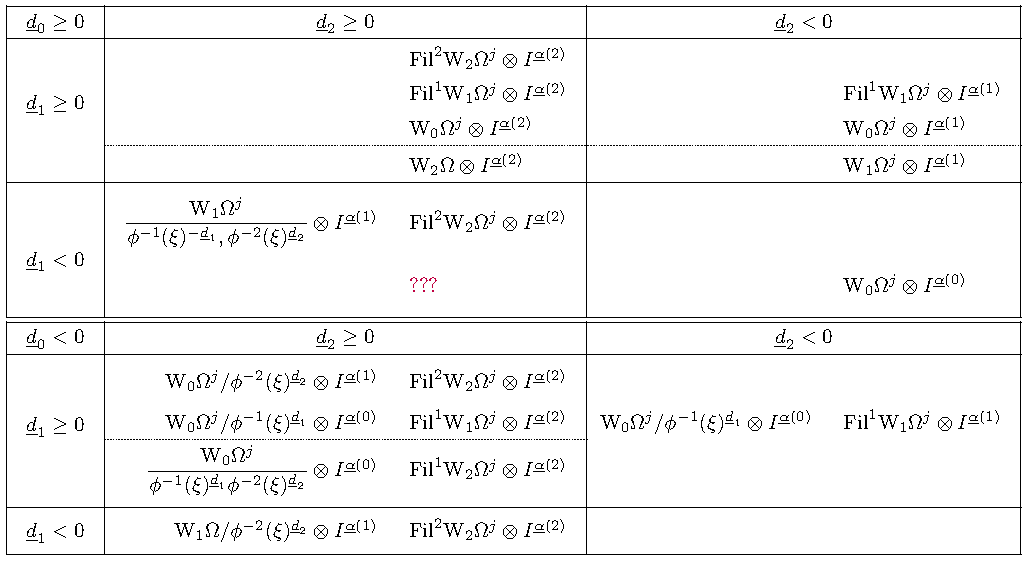
\includegraphics[width=\textwidth]{tables/hotrss-perfd.pdf}
    % \begin{tabular}{|c|r@{\hskip 1.5em}l|r@{\hskip 1.5em}l|}\hline
    %   \pad[1em] $\m d_0\ge0$ \rule[-.5em]{0pt}{.5em} & \multicolumn{2}{c|}{$\m d_2\ge0$} & \multicolumn{2}{c|}{$\m d_2<0$}\\\hline
    %   \multirow{4}{*}{$\m d_1\ge0$}
    %     && $\Fil^2\dRW[2]^j \tnsr I^{\m\alpha(2)}$ \pad[1.2em] &&\\[.2em]
    %     && $\Fil^1\dRW[1]^j \tnsr I^{\m\alpha(2)}$
    %     && $\Fil^1\dRW[1]^j \tnsr I^{\m\alpha(1)}$\\[.2em]
    %     && $\dRW[0]^j \tnsr I^{\m\alpha(2)}$
    %     && $\dRW[0]^j \tnsr I^{\m\alpha(1)}$\\[.4em]\cdashline{2-5}[.4pt/1pt]
    %     && $\dRW[2]\tnsr I^{\m\alpha(2)}$ && $\dRW[1]^j\tnsr I^{\m\alpha(1)}$ \pad[1.2em]\\[.2em]\hline
    %   \multirow{3}{*}{$\m d_1<0$}
    %     & \pad[1.8em] $\dfrac{\dRW[1]^j}{\phi^{-1}(\xi)^{-\m d_1},\phi^{-2}(\xi)^{\m d_2}}\tnsr I^{\m\alpha(1)}$
    %     & $\Fil^2\dRW[2]^j\tnsr I^{\m\alpha(2)}$ &&\\
    %     &&&&\\
    %     & & \color{purple}{???} && $\dRW[0]^j \tnsr I^{\m\alpha(0)}$\\[.4em]
    %     \hline\hline
    %   \pad[1em] $\m d_0<0$ \rule[-.5em]{0pt}{.5em} & \multicolumn{2}{c|}{$\m d_2\ge0$} & \multicolumn{2}{c|}{$\m d_2<0$}\\\hline
    %   \multirow{3}{*}{$\m d_1\ge0$}
    %     & $\dRW[0]^j/\phi^{-2}(\xi)^{\m d_2}\tnsr I^{\m\alpha(1)}$
    %     & $\Fil^2\dRW[2]^j \tnsr I^{\m\alpha(2)}$ \pad[1.2em]
    %     &&\\[.4em]
    %     & $\dRW[0]^j/\phi^{-1}(\xi)^{\m d_1}\tnsr I^{\m\alpha(0)}$
    %     & $\Fil^1\dRW[1]^j \tnsr I^{\m\alpha(2)}$
    %     & $\dRW[0]^j/\phi^{-1}(\xi)^{\m d_1}\tnsr I^{\m\alpha(0)}$
    %     & $\Fil^1\dRW[1]^j\tnsr I^{\m\alpha(1)}$\\[.4em]\cdashline{2-3}[.4pt/1pt]
    %     & \pad[1.8em] $\dfrac{\dRW[0]^j}{\phi^{-1}(\xi)^{\m d_1}\phi^{-2}(\xi)^{\m d_2}}\tnsr I^{\m\alpha(0)}$
    %     & $\Fil^1\dRW[2]^j\tnsr I^{\m\alpha(2)}$
    %     &&\\[1em]\hline
    %   $\m d_1<0$
    %     & $\dRW[1]/\phi^{-2}(\xi)^{\m d_2}\tnsr I^{\m\alpha(1)}$
    %     & $\Fil^2\dRW[2]^j \tnsr I^{\m\alpha(2)}$ \pad[1.2em] &&\\[.4em]\hline
    % \end{tabular}
    \caption{$E_\infty$ pages of the HOTRSS for $\TR^2_\rog(S\rel\SAinf{R^+})$. Extensions are marked below the dotted lines.}
  \end{center}
\end{figure}

\begin{figure}
  \label{fig:tr-cp2-crys}
  \begin{center}
    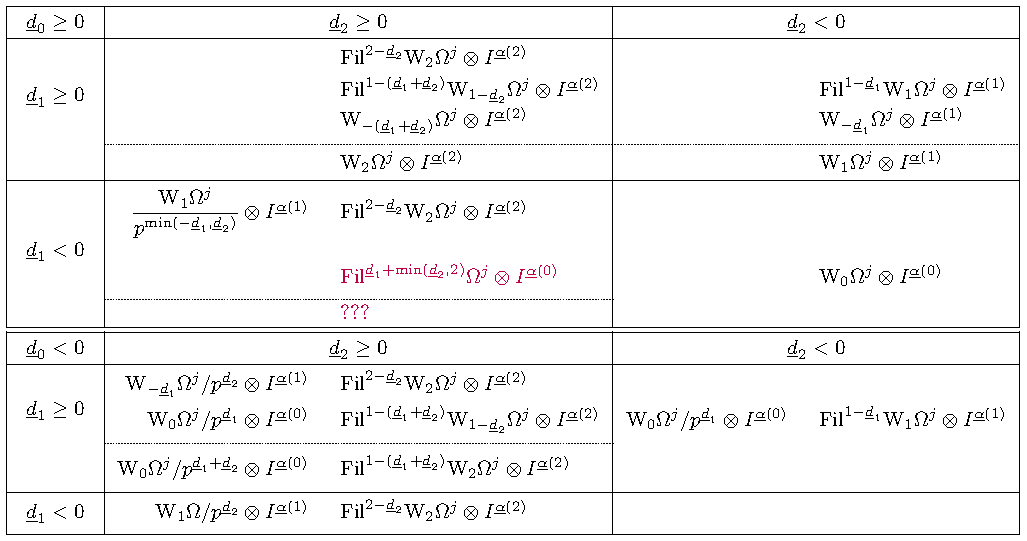
\includegraphics[width=\textwidth]{tables/hotrss-crys.pdf}
    % \begin{tabular}{|c|r@{\hskip 1.5em}l|r@{\hskip 1.5em}l|}\hline
    %   \pad[1em] $\m d_0\ge0$ \rule[-.5em]{0pt}{.5em} & \multicolumn{2}{c|}{$\m d_2\ge0$} & \multicolumn{2}{c|}{$\m d_2<0$}\\\hline
    %   \multirow{4}{*}{$\m d_1\ge0$}
    %     && $\Fil^{2-\m d_2}\dRW[2]^j \tnsr I^{\m\alpha(2)}$ \pad[1.2em] &&\\[.2em]
    %     && $\Fil^{1-(\m d_1+\m d_2)}\dRW[1-\m d_2]^j \tnsr I^{\m\alpha(2)}$
    %     && $\Fil^{1-\m d_1}\dRW[1]^j \tnsr I^{\m\alpha(1)}$\\[.2em]
    %     && $\dRW[-(\m d_1+\m d_2)]^j \tnsr I^{\m\alpha(2)}$
    %     && $\dRW[-\m d_1]^j \tnsr I^{\m\alpha(1)}$\\[.5em]\cdashline{2-5}[.4pt/1pt]
    %     && $\dRW[2]^j\tnsr I^{\m\alpha(2)}$ && $\dRW[1]^j\tnsr I^{\m\alpha(1)}$ \pad[1.2em]\\[.2em]\hline
    %   \multirow{4}{*}{$\m d_1<0$}
    %     & \pad[1.8em] $\dfrac{\dRW[1]^j}{p^{\min(-\m d_1,\m d_2)}}\tnsr I^{\m\alpha(1)}$
    %     & $\Fil^{2-\m d_2}\dRW[2]^j\tnsr I^{\m\alpha(2)}$ &&\\
    %     &&&&\\
    %     & & \color{purple}$\Fil^{\m d_1 + \min(\m d_2,2)}\Omega^j \tnsr I^{\m\alpha(0)}$ && $\dRW[0]^j \tnsr I^{\m\alpha(0)}$\\[.4em]\cdashline{2-3}[.4pt/1pt]
    %     && \pad[1em]\color{purple}{???} &&\\\hline\hline
    %   \pad[1em] $\m d_0<0$ \rule[-.5em]{0pt}{.5em} & \multicolumn{2}{c|}{$\m d_2\ge0$} & \multicolumn{2}{c|}{$\m d_2<0$}\\\hline
    %   \multirow{3}{*}{$\m d_1\ge0$}
    %     & $\dRW[-\m d_1]^j/p^{\m d_2}\tnsr I^{\m\alpha(1)}$
    %     & $\Fil^{2-\m d_2}\dRW[2]^j \tnsr I^{\m\alpha(2)}$ \pad[1.2em]
    %     &&\\[.4em]
    %     & $\dRW[0]^j/p^{\m d_1}\tnsr I^{\m\alpha(0)}$
    %     & $\Fil^{1-(\m d_1+\m d_2)}\dRW[1-\m d_2]^j \tnsr I^{\m\alpha(2)}$
    %     & $\dRW[0]^j/p^{\m d_1}\tnsr I^{\m\alpha(0)}$
    %     & $\Fil^{1-\m d_1}\dRW[1]^j\tnsr I^{\m\alpha(1)}$\\[.5em]\cdashline{2-3}[.4pt/1pt]
    %     & \pad $\dRW[0]^j/p^{\m d_1+\m d_2}\tnsr I^{\m\alpha(0)}$
    %     & $\Fil^{1-(\m d_1+\m d_2)}\dRW[2]^j\tnsr I^{\m\alpha(2)}$
    %     &&\\[.5em]\hline
    %   $\m d_1<0$
    %     & $\dRW[1]/p^{\m d_2}\tnsr I^{\m\alpha(1)}$
    %     & $\Fil^{2-\m d_2}\dRW[2]^j \tnsr I^{\m\alpha(2)}$ \pad[1.2em] &&\\[.4em]\hline
    % \end{tabular}
    \caption{$E_\infty$ pages of the HOTRSS for $\TR^2_\rog(S\rel\SW k)$. Extensions are marked below the dotted lines.}
  \end{center}
\end{figure}

\begin{proof}
  We begin with the easier case that $S$ is $p$-completely smooth over $R^+$.

  First we show that for $r\ge1$, the $E^r$ page of the HOTRSS is given by
  \begin{align*}
    E^r_{s,\m\alpha,j} &= \Fil^s\dRW[s]^j_{S/R^+} \tnsr I^{\m \alpha(\min(s+r-1,\ell))}\\
    %\bigotimes_{i=0}^{\min(s+r-1, \ell)} (\phi^{-i}(\xi) A)^{\tnsr\m d_i}\\
    E^r_{s,\m\alpha-1,j} &= \frac{\dRW[\max(s-r,k-1)]^j_{S/R^+}}{\phi^{-s}(\xi)^{\m d_s}} \tnsr I^{\m\alpha(s-1)}%\bigotimes_{i=0}^{s-1} (\phi^{-i}(\xi) A)^{\tnsr \m d_i}
  \end{align*}

  The $E^0$ page is given by
  \[
    E^0_{s,\m\alpha-*,j} =
    \left(\xymatrix@1{
        \ds\dRW[s-1]^j_{S/R^+} \tnsr I^{\m\alpha(s-1)}%\bigotimes_{i=0}^{s-1} (\phi^{-i}(\xi)A)^{\tnsr \m d_i}
        &
        \ar[l]
        \ds\dRW[s]^j_{S/R^+} \tnsr I^{\m\alpha(s)}%\bigotimes_{i=0}^s (\phi^{-i}(\xi)A)^{\tnsr \m d_i}
      }\right)
      \quad k\le s\le \ell
  \]
  from which we see that the $E^1$ page is as claimed. Inductively, on page $E^r$ there are differentials
  \[\xymatrix@C=-15em@R=1em{
      *!R{\fade{[s+r\le\ell]\left(\ds\frac{\dRW[s]^j_{S/R^+}}{\fade[100]{\phi^{-(s+r)}(\xi)^{\m d_{(s+r)}}}} \tnsr I^{\m\alpha(s+r-1)}
            %\bigotimes_{i=0}^{s+r-1} (\phi^{-i}(\xi) A)^{\tnsr \m d_i}
      \right)}}\\
      *!R{\left(\ds\frac{\dRW[s-r]^j_{S/R^+}}{\phi^{-s}(\xi)^{\m d_s}} \tnsr
          I^{\m\alpha(s-1)}
 %     \bigotimes_{i=0}^{s-1} (\phi^{-i}(\xi) A)^{\tnsr \m d_i}
  \right)}
     & *!L{\ \ds\Fil^s \dRW[s]^j_{S/R^+} \tnsr
       I^{\m\alpha(s+r-1)}
  %   \bigotimes_{i=0}^{s+r-1} (\phi^{-i}(\xi) A)^{\tnsr\m d_i}
   } \ar[ul]\\
     & *!L{\fade{\left(\ds\fade[100]{\Fil^{s-r}} \dRW[s-r]^j_{S/R^+} \tnsr
           I^{\m\alpha(s-1)}
%     \bigotimes_{i=0}^{s-1} (\phi^{-i}(\xi) A)^{\tnsr\m d_i}
\right)[k\le s-r]}}
     \ar[ul]
  }\]
  where we use the Iverson bracket to denote that the terms may be zero. Since $\m\alpha$ is contiguous, the terms stabilize as soon as the target/source of the relevant differential vanishes. From this we see that the $E^{r+1}$ page is as claimed.

  Now we have
  \begin{alignat*}2
    E^\infty_{s,\m\alpha,j} &= \Fil^s\dRW[s]^j_{S/R^+} \tnsr
    I^{\m\alpha(\ell)}
    %\bigotimes_{i=0}^\ell (\phi^{-i}(\xi) A)^{\tnsr\m d_i}
                            &\qquad& k\le s\le\ell\\
    E^\infty_{s,\m\alpha-1,j} &= \frac{\dRW[k-1]^j_{S/R^+}}{\phi^{-s}(\xi)^{\m d_s}} \tnsr
    I^{\m\alpha(s-1)}
    %\bigotimes_{i=0}^{s-1} (\phi^{-i}(\xi) A)^{\tnsr \m d_i}
                              && k \le s\le\ell
  \end{alignat*}
  from which the extensions are clear.

  Now we tackle the harder case that $S$ is smooth over $k$. Let $\hat r=\min(r,\ell-s+1)$ and let $\check r=\min(r,s-k+1)$. First we show that for $r\ge1$, the $E^r$ page of the HOTRSS is given by
  \begin{align*}
    E^r_{s,\m\alpha,j} &= \Fil^{s-\sum_{i=s}^{s+\hat r-1}\m d_i}\dRW[[s-\sum_{i=s+1}^{s+\hat r-1}\m d_i{]}]^j_S \tnsr 
   I^{\m\alpha(s+\hat r-1)}
    %\left(p^{\sum_{i=0}^{s+\hat r-1}\m d_i}\rmW\right)
    \\
    E^r_{s,\m\alpha-1,j} &= \frac{\dRW[[s-\check r-\sum_{i=s-\check r+1}^{s-1} \m d_i{]}]^j_S}{p^{\m d_s}} \tnsr
    I^{\m\alpha(s-1)}
    %\left(p^{\sum_{i=0}^{s-1}\m d_i}\rmW\right)
  \end{align*}

  The $E^0$ page is given ($k\le s\le \ell$) by
  \begin{align*}
    E^0_{s,\m\alpha-*,j} &=
    \left[\xymatrix@1{
        \ds\dRW[s-1]^j_S \tnsr
        I^{\m\alpha(s-1)}
        %\left(p^{\sum_{i=0}^{s-1}\m d_i}\rmW\right)
        &
        \ar[l]
        \ds\dRW[s]^j_S \tnsr
        I^{\m\alpha(s)}
        %\left(p^{\sum_{i=0}^s\m d_i}\rmW\right)
      }\right]
      \\
      \intertext{from which we see that the $E^1$ page is}
      E^1_{s,\m\alpha-*,j} &=
        \left[\xymatrix@1{
                \ds\frac{\dRW[s-1]^j_S}{p^{\m d_s}} \tnsr
                I^{\m\alpha(s-1)}
                %\left(p^{\sum_{i=0}^{s-1}\m d_i}\rmW\right)
                &
                \ds\Fil^{s-\m d_s}\dRW[s]^j_S \tnsr
                I^{\m\alpha(s)}
               % \left(p^{\sum_{i=0}^s\m d_i}\rmW\right)
  }\right]
  \end{align*}
  as claimed. Inductively, on page $E^r$ there are differentials
  \small\[\hspace{-2em}\xymatrix@C=-22em@R=1em{
      *!R{\fade{[s+r\le\ell]\left(\ds\frac{\dRW[[s-\sum_{i=s+1}^{s+r-1}\m d_i{]}]^j_S}{\fade[100]{p^{\m d_{(s+r)}}}} \tnsr
            I^{\m\alpha(s+r-1)}
      %\left(p^{\sum_{i=0}^{s+r-1}\m d_i}\rmW\right)
\right)}}\\
      *!R{\left(\ds\frac{\dRW[[s-r-\sum_{i=s-r+1}^{s-1}\m d_i{]}]^j_S}{p^{\m d_s}} \tnsr
          I^{\m\alpha(s-1)} %\left(p^{\sum_{i=0}^{s-1}\m d_i}\rmW\right)
  \right)}
     & *!L{\ \ds\Fil^{s - \sum_{i=s}^{s+r-1}\m d_i} \dRW[[s-\sum_{i=s+1}^{s+r-1}\m d_i{]}]^j_S \tnsr
       I^{\m\alpha(s+r-1)} %\left(p^{\sum_{i=0}^{s+r-1}\m d_i}\rmW\right)
   } \ar[ul]\\
     & *!L{\fade{\left(\ds\fade[100]{\Fil^{s-r-\sum_{i=s-r}^{s-1}\m d_i}} \dRW[[s-r-\sum_{i=s-r+1}^{s-1}\m d_i{]}]^j_S \tnsr
           I^{\m\alpha(s-1)} %\left(p^{\sum_{i=0}^{s-1}\m d_i}\rmW\right)
     \right)[k\le s-r]}}
     \ar[ul]
}\]\normalsize
where we use the Iverson bracket to denote that the terms may be zero. Since $\m\alpha$ is contiguous, the terms stabilize as soon as the target/source of the relevant differential vanishes. From this we see that the $E^{r+1}$ page is as claimed.

  Now we have
  \begin{alignat*}2
    E^\infty_{s,\m\alpha,j} &= \Fil^{s-\sum_{i=s}^\ell \m d_i}\dRW[[s-\sum_{i=s+1}^\ell \m d_i{]}]^j_S \tnsr
    I^{\m\alpha(\ell)}%\left(p^{\sum_{i=0}^\ell \m d_i}\rmW\right)
                            &\qquad& k\le s\le\ell\\
    E^\infty_{s,\m\alpha-1,j} &= \frac{\dRW[[k-1-\sum_{i=k}^{s-1}\m d_i{]}]^j_S}{p^{\m d_s}} \tnsr
    I^{\m\alpha(s-1)}%\left(p^{\sum_{i=0}^{s-1}\m d_i}\rmW\right)
                              && k \le s\le\ell
  \end{alignat*}
  from which the extensions are clear.
\end{proof}

\subsection{Special cases}
\label{sub:special}

Here we record some special cases of the theorem that are of interest for applications. In the positive and negative ranges, it is often more convenient to work with coefficients of irreducible decompositions rather than with dimension sequences. Note that there is some redundancy in the following statements since the integer grading $2i$ could be absorbed into $\m d_0$; we have phrased them this way since in applications one usually fixes $\m\alpha$ and considers $\TR_{2i\pm\m\alpha}$ for varying $i$.

\begin{corollary}[Negative range]
  Let $\m\alpha = \sum_{r=0}^n \m c_r \m\lambda_r$ be an actual poly-representation. Given $i\ge0$, let $\ell$ be such that
  \[ i - \m d_{\ell+1}(\m\alpha) < 0 \le i-\m d_\ell(\m\alpha). \]

  Then if $S$ is $p$-completely smooth over an arbitrary perfectoid ring $R$, we have
  \begin{align*}
    \TR^n_{2i-\m\alpha,j}(S;\Z_p)
      &= \dRW[\ell]^j_{S/R} \tnsr \bigotimes_{r=0}^\ell \phi^{-r}(\xi)^{i-\m d_r}A\\
      &= \dRW[\ell]^j_{S/R} \tnsr \xi_{\ell+1}^iA \tnsr \bigotimes_{r=0}^\ell \phi^{-r}(\xi_{\ell+1-r})^{-\m c_r}A\\
    \TR^n_{(2i-\m\alpha)-1,j}(S;\Z_p) &= 0
  \end{align*}
\end{corollary}
\begin{proof}
  When $R$ is either a perfect $\F_p$-algebra or $p$-torsionfree, we apply Theorem \ref{thm:tr-ctg}. For this, note that the polyrepresentation $2i-\m\alpha$ is non-negatively concentrated in $[-\ell,0]$, and $\m d_r(\alpha) = \sum_{s=0}^r \m c_r$. Since the result is the same in both cases, it must be true for arbitrary perfectoid rings using the fracture square of \cite[Proposition IV.3.2]{PrismNotes}.
\end{proof}

\begin{corollary}[Positive range]
  Let $\m\alpha = \sum_{r=0}^n \m c_r \m\lambda_r$ be an actual polyrepresentation. Given $i\in\Z$, let $k=k(i)$ be such that
  \[ \m d_{(k-1)}(\m\alpha) - i < 0 \le \m d_k(\m\alpha) - i. \]

  If $S$ is $p$-completely smooth over a $p$-torsionfree perfectoid ring $R^+$, then there are canonical identifications
  \begin{align*}
    \TR^n_{\m\alpha-2i,j}(S\rel\SAinf{R^+})
      &= \Fil^k \dRW[n]^j_{S/R^+} \tnsr \bigotimes_{r=0}^n \phi^{-r}(\xi)^{\m d_r-i}A\\
      &= \Fil^k \dRW[n]^j_{S/R^+} \tnsr (\xi_{n+1} A)^{-i} \tnsr \bigotimes_{r=0}^n \phi^{-r}(\xi_{n+1-r})^{\m c_r} A\\
      \TR^n_{(\m\alpha-2i)-1,j}(S\rel\SAinf{R^+})
      &= \frac{\dRW[k-1]^j_{S/R^+}}{\phi^{-k}(\xi)^{\m d_k-i}\dotsm\phi^{-n}(\xi)^{\m d_n-i}}\tnsr\bigotimes_{r=0}^{k-1} \phi^{-r}(\xi)^{\m d_r-i}A\\
      &= \frac{\dRW[k-1]^j_{S/R^+}}{\ds\frac1{\phi^{-k}(\xi_{n+1-k})^i}\prod_{r=k}^n \phi^{-r}(\xi_{n+1-r})^{\m c_r}} \tnsr (\xi_k A)^{-i} \tnsr \bigotimes_{r=0}^{k-1} \phi^{-r}(\xi_{k-r})^{\m c_r} A
  \end{align*}
  Using the first form, this also holds for $n=\infty$ if $R^+=\O_C$.

  If $S$ is smooth over a perfect $\F_p$-algebra $k$, then there are canonical identifications
  \begin{align*}
    \TR^n_{\m\alpha-2i,j}(S\rel\SW k)
      &= \Fil^{k - \left[\sum_{r=k}^n (\m d_r - i) \right]} \dRW[n]^j_S\tnsr p^{\left[\sum_{r=0}^n (\m d_r - i) \right]}W\\
      &= \Fil^{k - \left[\sum_{r=k}^n (n+1-r)\m c_r\right] + (n-k+1)i} \dRW[n]^j_S\tnsr p^{\left[\sum_{r=0}^n (n+1-r)\m c_r\right] - (n+1)i}W\\
    \TR^n_{\m\alpha-2i-1,j}(S\rel\SW k)
      &= \frac{\dRW[k-1]^j_S}{p^{\left[\sum_{r=k}^n (\m d_r-i)\right]}}\tnsr p^{\left[\sum_{r=0}^{k-1} (\m d_r-i)\right]}W\\
      &= \frac{\dRW[k-1]^j_S}{p^{\left[\sum_{r=k}^n (n+1-r)\m c_r\right]-(n+1-k)i}}\tnsr p^{\left[\sum_{r=0}^{k-1}(k-r)\m c_r\right]-ki}W
  \end{align*}
  This also holds for $n=\infty$ using the first form.
\end{corollary}

\begin{corollary}
  Let $\m\alpha$ be an actual poly-representation with $\m d_0(\m\alpha)\ge i$. If $S$ is $p$-completely smooth over an arbitrary perfectoid ring $R$, then there are canonical identifications
  \begin{align*}
    \TR^n_{\m\alpha-2i,j}(S\rel\SAinf{R})
      &= \dRW[n]^j_{S/R} \tnsr \bigotimes_{r=0}^n \phi^{-r}(\xi)^{\m d_r-i}A\\
      &= \dRW[n]^j_{S/R} \tnsr (\xi_{n+1} A)^{-i } \tnsr \bigotimes_{r=0}^n\phi^{-r}(\xi_{n-r+1})^{\m c_r}A\\
      \TR^n_{\m\alpha-2i-1,j}(S\rel\SAinf{R})
      &= 0
  \end{align*}
  Using the first form, this also holds for $n=\infty$ if $n<\infty$ or if $R\in\{k,\O_C\}$.
\end{corollary}

Here is the only other infinite-level computation where we know how to control the limit.

\begin{corollary}[Eventually constant contiguous range]
  Let $\m\alpha$ be a $\Z_p$-polyrepresentation non-negatively concentrated in $(-\infty,-k]$, and suppose that $\m d_r=\m d_\ell$ for all $r\ge\ell$.

  If $S$ is $p$-completely smooth over $\O_C$, then
  \begin{align*}
    \TR_{\m\alpha,j}(S\rel\SAinf{\O_C})
      &= \Fil^k \dRW^j_{S/\O_C} \tnsr \left(\bigotimes_{i=0}^{\ell-1} \phi^{-i}(\xi)^{\m d_i}A\right) \tnsr \left(\phi^{-\ell}(\mu)^{\m d_\ell}A\right)\\
      \TR_{\m\alpha-1,j}(S\rel\SAinf{\O_C})
      &= \frac{\dRW[k-1]^j_{S/\O_C}}{\phi^{-\ell}(\mu)^{\m d_\ell}\prod_{i=0}^{\ell-1}\phi^{-i}(\xi)^{\m d_i}} \tnsr\bigotimes_{i=0}^{k-1} \phi^{-i}(\xi)^{\m d_i}A
  \end{align*}

  If $S$ is smooth over $k$,
  \begin{align*}
    \TR_{\m\alpha,j}(S\mid\SW k)
      &= \begin{cases}
        \Fil^{k-(\m d_k+\dotsb+\m d_{\ell-1})} \dRW^j_S\tnsr \left(p^{\m d_0 + \dotsb + \m d_{\ell-1}}W\right) & \m d_\ell = 0\\
        0 & \m d_\ell > 0
      \end{cases}\\
    \TR_{\m\alpha-1,j}(S\mid\SW k)
      &= \left\{\!\!\!
        \begin{array}{r@{}ll}
          \dfrac{\dRW[k-1]^j_S}{p^{\m d_k+\dotsb + \m d_{\ell-1}}} &{}\tnsr \left(p^{\m d_0 + \dotsb + \m d_{(k-1)}}W\right) & \m d_\ell = 0\\
          \dRW[k-1]^j_S &{}\tnsr \left(p^{\m d_0 + \dotsb + \m d_{(k-1)}}W\right) & \m d_\ell >0
        \end{array}
        \right.
  \end{align*}
\end{corollary}

